\documentclass[a4paper,twoside,11pt]{article}
\usepackage{a4wide,graphicx,fancyhdr,amsmath,amssymb}
\usepackage{algorithmic}

%----------------------- Macros and Definitions --------------------------

\setlength\headheight{20pt}
\addtolength\topmargin{-10pt}
\addtolength\footskip{20pt}

\newcommand{\N}{\mathbb{N}}
\newcommand{\ch}{\mathcal{CH}}
\everymath{\displaystyle}
\newcommand{\solution}[1]{\noindent{\bf Solution to Exercise #1:}}

\fancypagestyle{plain}{%
\fancyhf{}
\fancyhead[LO,RE]{\sffamily\bfseries\large Technische universiteit Eindhoven}
\fancyhead[RO,LE]{\sffamily\bfseries\large 2IV35 Visualization}
\fancyfoot[LO,RE]{\sffamily\bfseries\large department of mathematics and computer science}
\fancyfoot[RO,LE]{\sffamily\bfseries\thepage}
\renewcommand{\headrulewidth}{0pt}
\renewcommand{\footrulewidth}{0pt}
}

\pagestyle{fancy}
\fancyhf{}
\fancyhead[RO,LE]{\sffamily\bfseries\large Technische universiteit Eindhoven}
\fancyhead[LO,RE]{\sffamily\bfseries\large 2IV35 Visualization}
\fancyfoot[LO,RE]{\sffamily\bfseries\large department of mathematics and computer science}
\fancyfoot[RO,LE]{\sffamily\bfseries\thepage}
\renewcommand{\headrulewidth}{1pt}
\renewcommand{\footrulewidth}{0pt}

%-------------------------------- Title ----------------------------------

\title{\vspace{-\baselineskip}\sffamily\bfseries 2IV35 Visualization Set 2}
\author{Jeroen van Oorschot \qquad Student number: 0721913 \\{\tt j.v.oorschot@student.tue.nl}}

\date{\today}

%--------------------------------- Text ----------------------------------

\begin{document}
\maketitle

\pagebreak
\tableofcontents
\newpage
\section{Volume Rendering}
\subsection{Tri-linear interpolation}
To make sure we can also get data from between points we want to do some interpolation on the data. So I use the following function to get a value on point $(x,y,z)$ in a field $F$ with the value $F[i][j][k]$ for the integer values $i$, $j$ and $k$ by calculating the value $val$ with:
\begin{eqnarray*}
\alpha =& x-\lfloor x \rfloor\\
\beta =& y-\lfloor y \rfloor\\
\gamma =& z-\lfloor z \rfloor\\
val =& (1 - \alpha) * (1 - \beta) * (1 - \gamma ) * F[\lfloor x \rfloor][\lfloor y \rfloor][\lfloor z \rfloor] \\
&+ \alpha * (1 - \beta) * (1 - \gamma ) * F[\lceil x \rceil][\lfloor y \rfloor][\lfloor z \rfloor]\\
                    &+ (1 - \alpha) * \beta * (1 - \gamma ) * F[\lfloor x \rfloor][\lceil y \rceil][\lfloor z \rfloor] \\
                    &+ \alpha * \beta * (1 - \gamma ) * F[\lceil x \rceil][\lceil y \rceil][\lfloor z \rfloor]\\
                    &+ (1 - \alpha) * (1 - \beta) * \gamma  * F[\lfloor x \rfloor][\lfloor y \rfloor][\lceil z \rceil] \\
                    &+ \alpha * (1 - \beta) * \gamma  * F[\lceil x \rceil][\lfloor y \rfloor][\lceil z \rceil]\\
                    &+ (1 - \alpha) * \beta * \gamma  * F[\lfloor x \rfloor][\lceil y \rceil][\lceil z \rceil] \\
                    &+ \alpha * \beta * \gamma  * F[\lceil x \rceil][\lceil y \rceil][\lceil z \rceil]
\end{eqnarray*}
\subsection{Gaining speed}
I implemented two ways to speed up my program a bit, one is by making a low and a high resolution maximum intensity projection(MIP), in the low resolution (in my program just called MIP) we start at one and take steps of two in calculating pixel colour, while making pixels $(x,y)$,$(x-1,y)$,$(x,y-1)$ and $(x-1,y-1)$ all that color. I also added the possibility to manually adjust the number of samples. Results of tests on the backpack dataset can be found in this table, the numbers represent the rendering time in ms:
\begin{center}
  \begin{tabular}{| l || r | r | }
    \hline
    samples & hi & low \\ \hline
    223 & 11904 & 2933 \\ \hline
    22 & 1280 & 372 \\
    \hline
  \end{tabular}
\end{center}

\section{Maximum intensity projection}
In maximum intensity projection (MIP) we traverse trough the data and project at the point where that ray hits the screen the maximum of the samples on that ray. After implementing maximum intensity projection I opened all of the data sets with it to see the results.
\subsection{Backpack}
This worked fine, it was easy to see there was something like a bullet, a drug needle, a Swiss army knife and a spray can in the backpack, so this is suitable for an airport, because we can pick out the backs worth examining. Without hoovering around its less clear but a picture is included in Figure \ref{MB}.
\begin{figure}[!h]
  \centering
  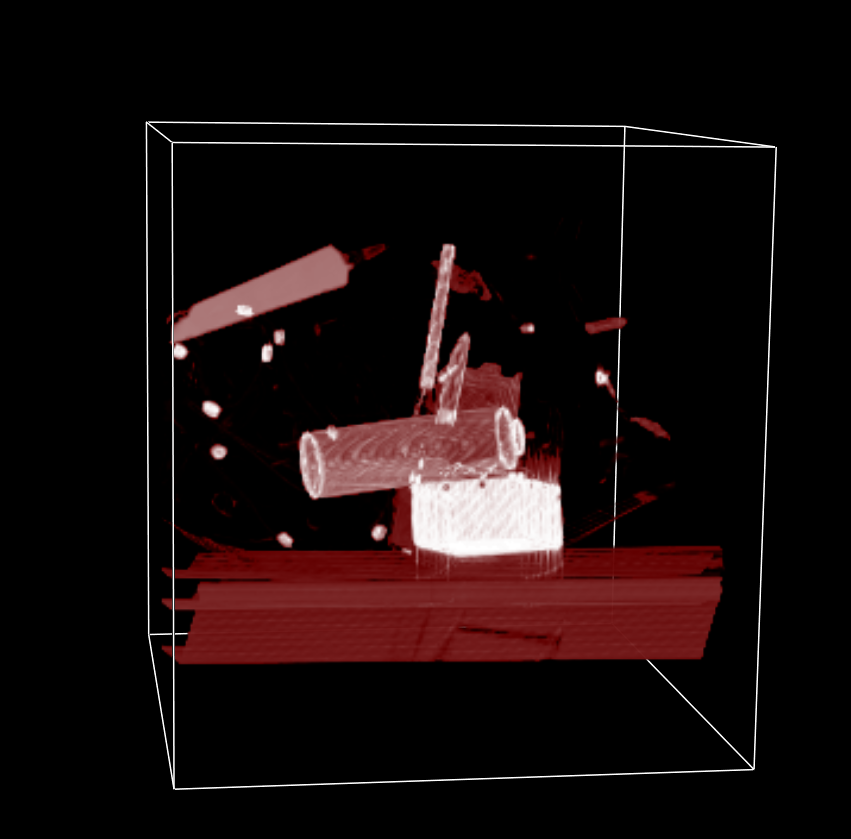
\includegraphics[width=0.5\textwidth]{MB.png}
  \caption{Resulting picture for backpack with MIP}
  \label{MB}
\end{figure}
\subsection{Bonsai}
This worked ok, we could see there was a tree. A picture is included in Figure \ref{MBon}.
\begin{figure}[!h]
  \centering
  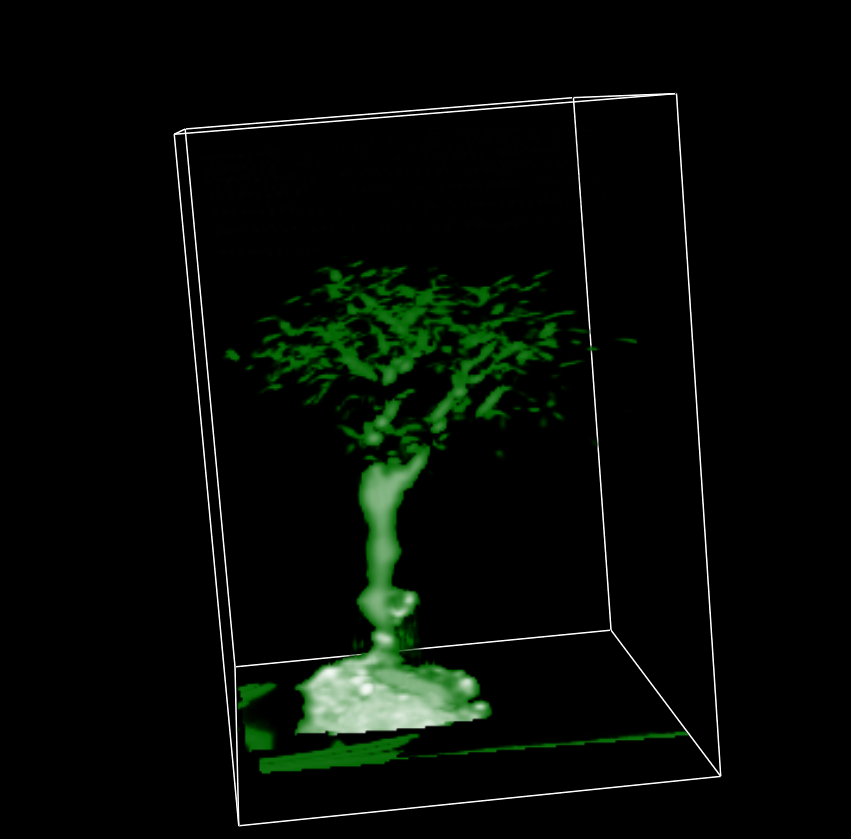
\includegraphics[width=0.5\textwidth]{MBon.png}
  \caption{Resulting picture for Bonsai with MIP}
  \label{MBon}
\end{figure}
\subsection{Carp}
This worked fantastic, we could see all the bones in the carp. A picture of the tail is included in Figure \ref{MCT}, the side is in Figure \ref{MCS}.
\begin{figure}[!h]
  \centering
  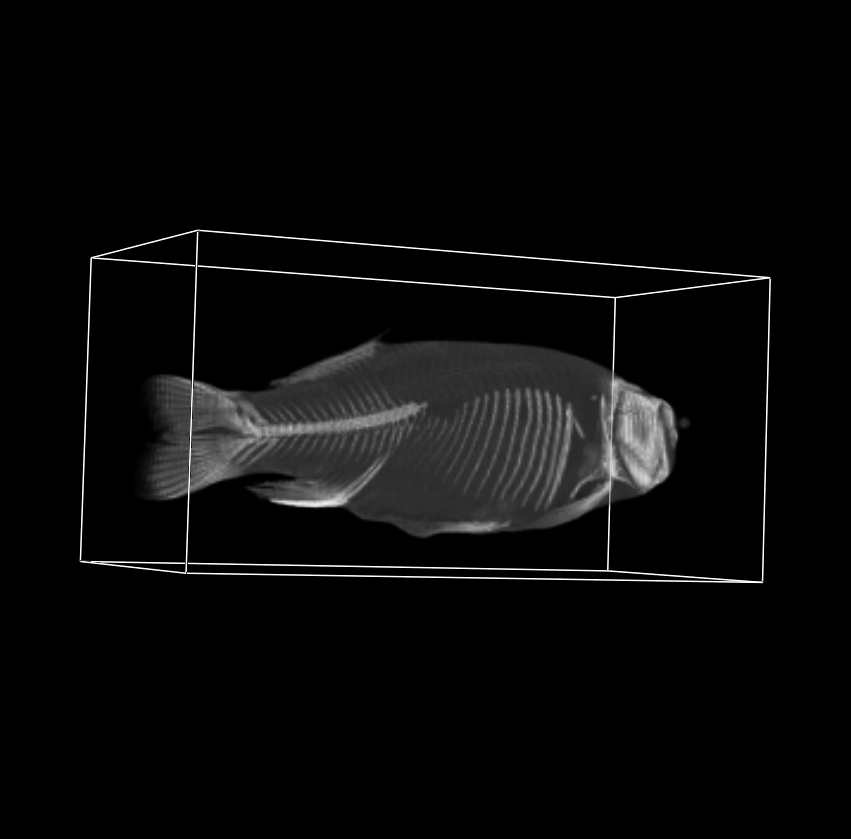
\includegraphics[width=0.5\textwidth]{MCT.png}
  \caption{Resulting picture for tail of the carp with MIP}
  \label{MCT}
\end{figure}
\begin{figure}[!h]
  \centering
  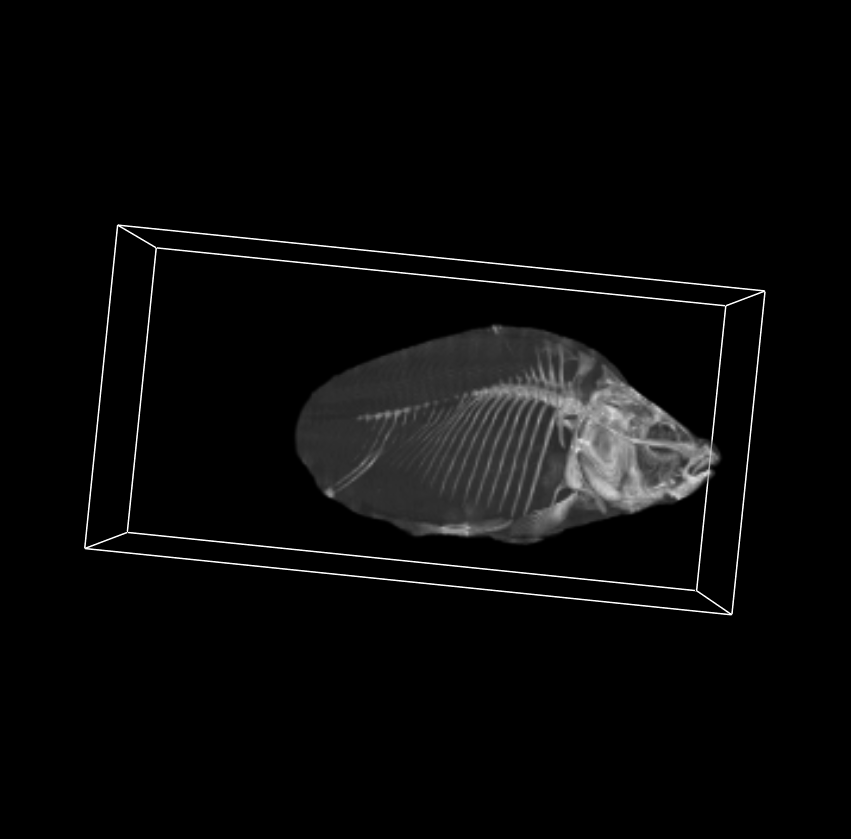
\includegraphics[width=0.5\textwidth]{MCS.png}
  \caption{Resulting picture for side of the carp with MIP}
  \label{MCS}
\end{figure}

\subsection{Orange}
This worked also good, I even was able to give the peel an orange color, while giving the inside a bleu color. A picture is included in Figure \ref{MO}.
\begin{figure}[!h]
  \centering
  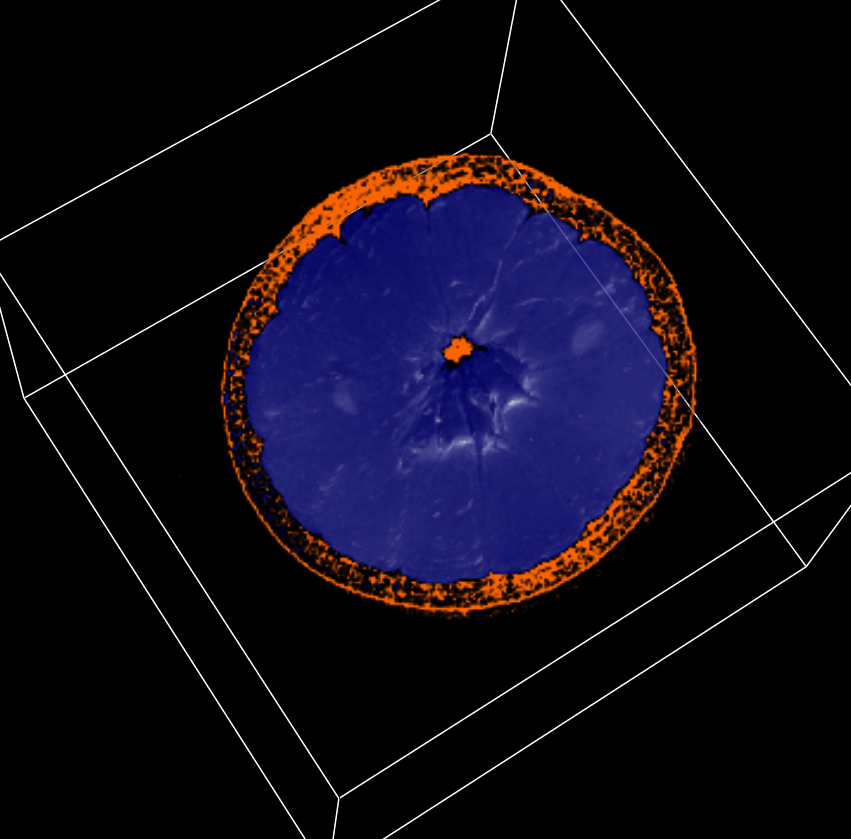
\includegraphics[width=0.5\textwidth]{MO.png}
  \caption{Resulting picture for orange with MIP}
  \label{MO}
\end{figure}

\subsection{Pig}
In this example I was able so show the coins in yellow and the pig in pink, also the hole is visible. A picture is included in Figure \ref{MP}.
\begin{figure}[!h]
  \centering
  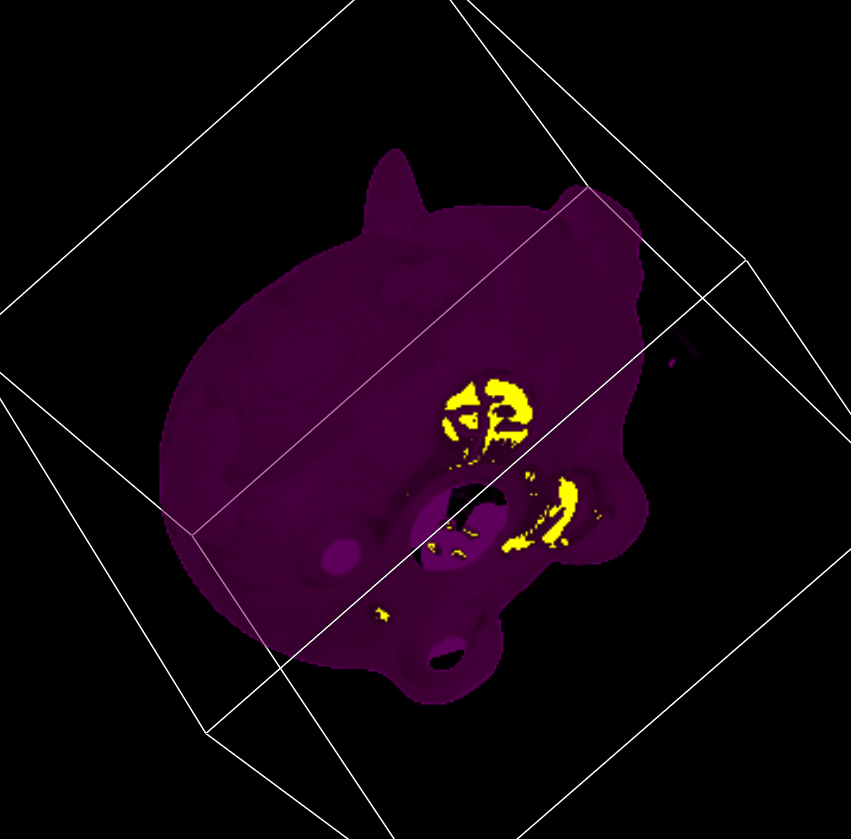
\includegraphics[width=0.5\textwidth]{MP.png}
  \caption{Resulting picture for pig with MIP}
  \label{MP}
\end{figure}

\subsection{Human}
Again a clear picture of a skeleton. A picture is included in Figure \ref{MH}.
\begin{figure}[!h]
  \centering
  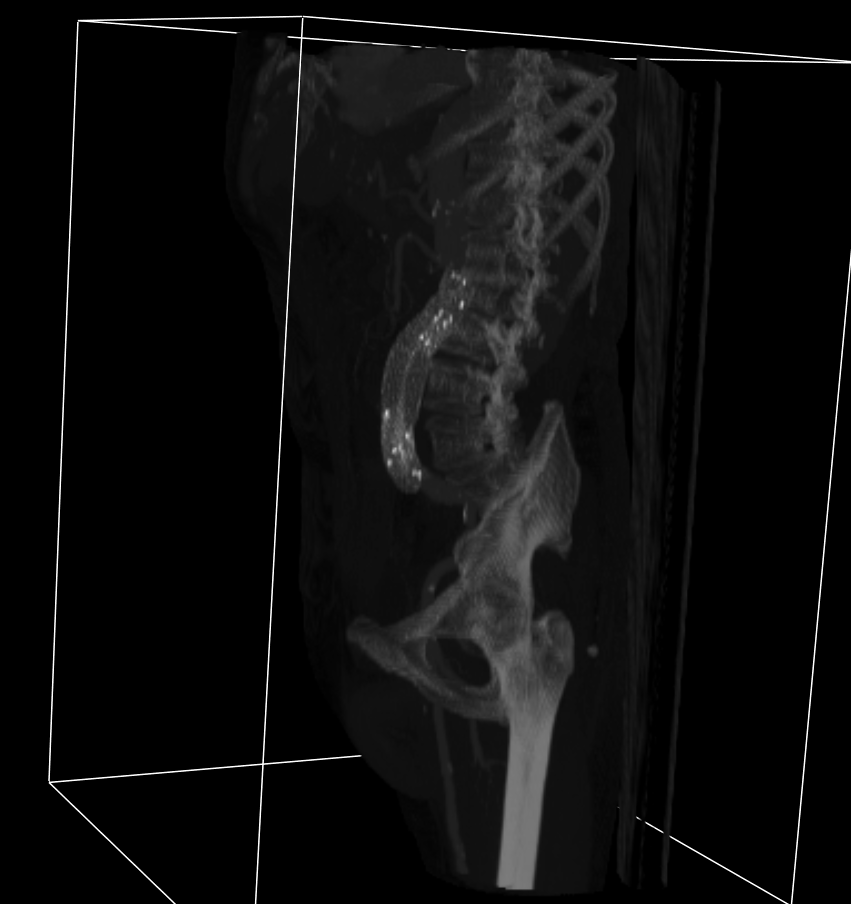
\includegraphics[width=0.5\textwidth]{MH.png}
  \caption{Resulting picture for human with MIP}
  \label{MH}
\end{figure}

\subsection{Tomato}
Since the tomato was not that nice on picture because its quite homogeneous and quite similar to the orange I decided to not include a picture for this.

\subsection{Tooth}
The tooth was also shown nice. A picture is included in Figure \ref{MT}.
\begin{figure}[!h]
  \centering
  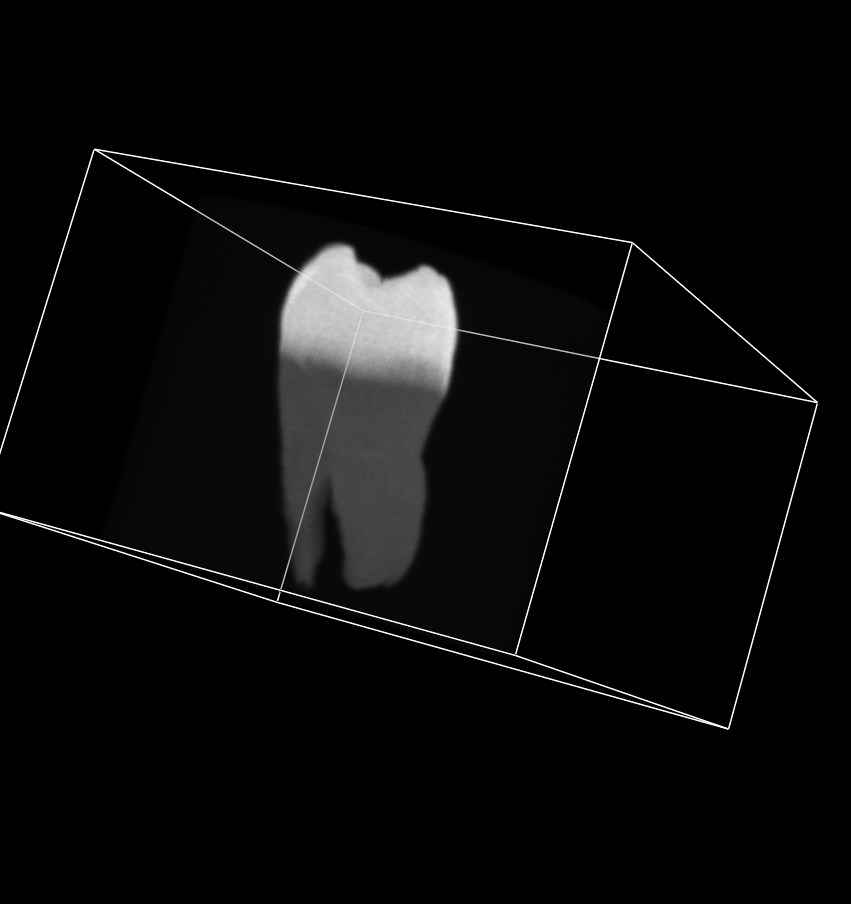
\includegraphics[width=0.5\textwidth]{MT.png}
  \caption{Resulting picture for tooth with MIP}
  \label{MT}
\end{figure}


\section{Transfer function}
In the transfer function I made at every sample $i$ the color $C_i$ is calculated, but there is also added a bit of the color $C_{i-1}$ behind it. This is done with the function $C_i = C(i)+ (1-\tau)C_{i-1}$.
 \subsection{Carp}
 Because its more dificult to find the correct colours I only included one picture in Figure \ref{hi}. It is nice to see the difference between the different tissues, we can see the green skin, the yellow brains, the red muscles and the grey bones.

\begin{figure}[!h]
  \centering
  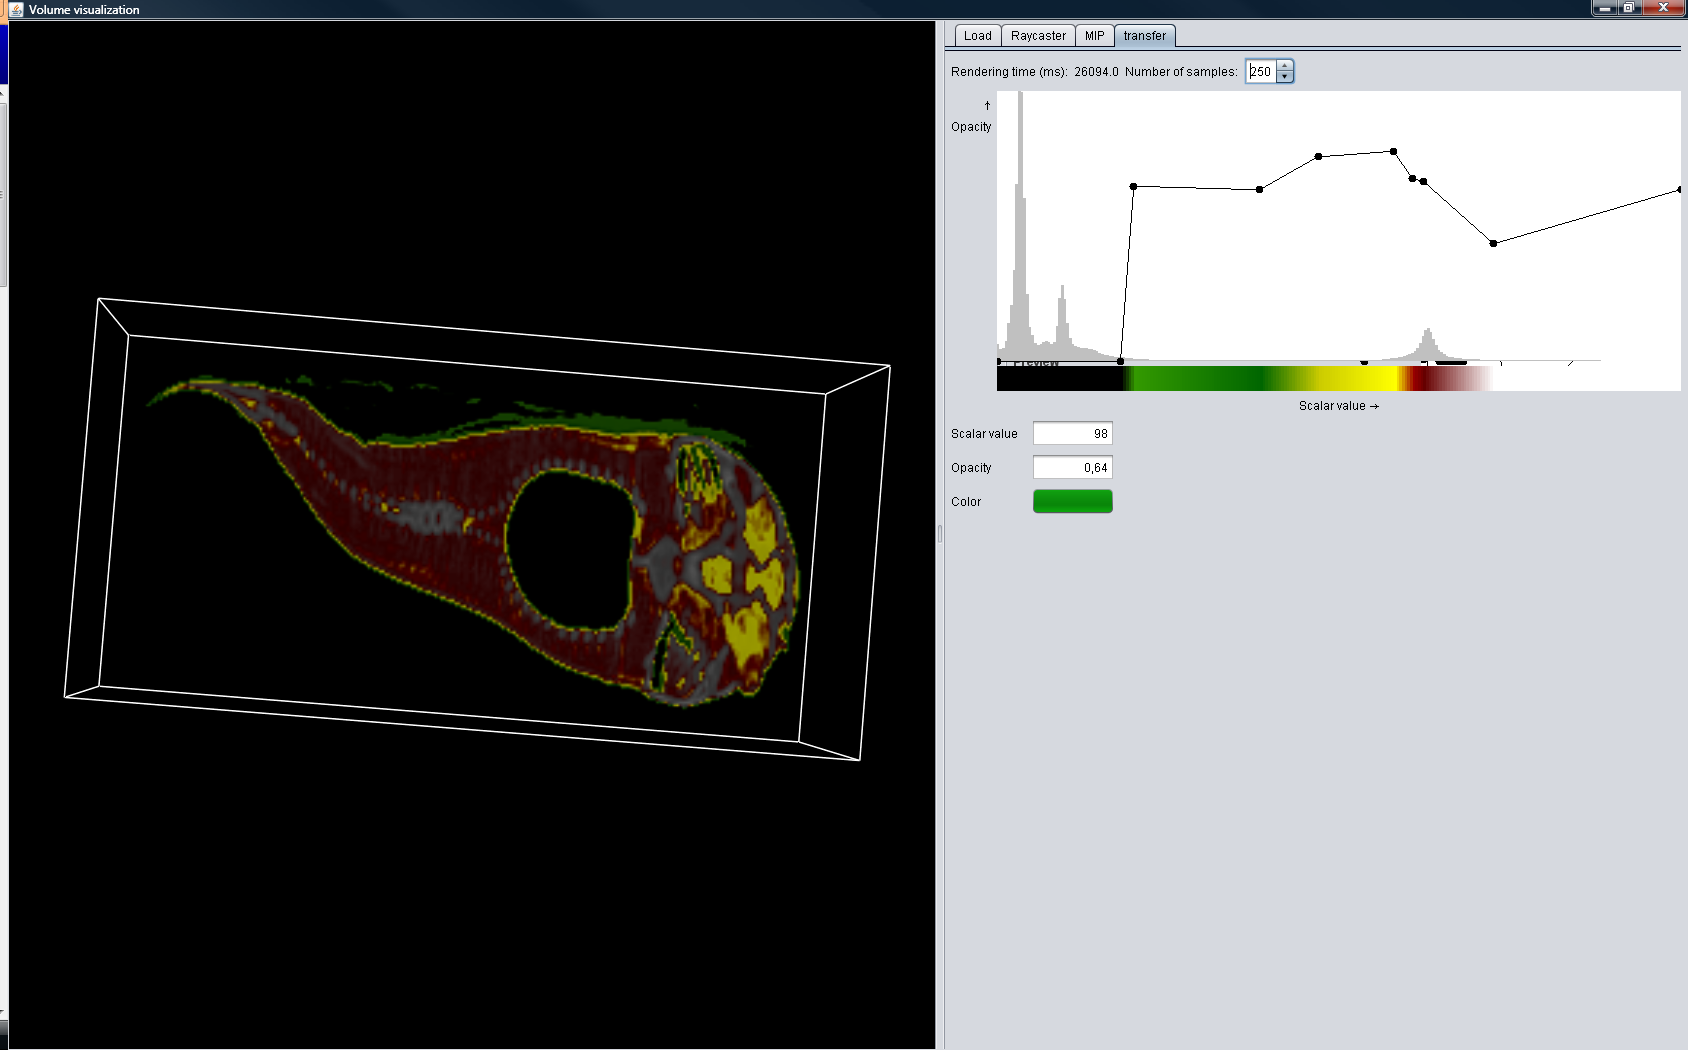
\includegraphics[width=1\textheight, angle=90]{hicarp.png}
  \caption{Resulting picture for the carp with transfer function}
  \label{hi}
\end{figure}
\end{document}
\subsection{Backpack}

\end{document}
